%Slask-innehållet i rapportmallen.

\section{Lorem ipsum dolor sit amet...}
\label{sec:loremipsum}

\nyterm{Lorem ipsum dolor sit amet}{Lorem ipsum dolor sit amet, consectetuer adipiscing elit\cite{loremipsum}.}, consectetuer adipiscing elit\cite{loremipsum}. Proin erat urna, condimentum et, sollicitudin eget, tempus quis, purus. Vestibulum a nisl. Nulla aliquet. Vivamus accumsan. Aenean cursus varius tellus. Maecenas nibh purus, lacinia id, auctor ac, sollicitudin et, magna. Donec lorem ipsum, facilisis sed, consequat porttitor, euismod pulvinar, ante. Mauris venenatis diam sed ligula. Proin justo. Quisque congue posuere est. Class aptent taciti sociosqu ad litora torquent per conubia nostra, per inceptos hymenaeos.

\section{Figurer, tabeller och annat}

\subsection{Trädstrukturer}
\label{subsec:trees}

Paketet \texttt{qtree} tillåter att man ritar träd. Paketet är mycket
syntax-känsligt, men det går att göra en del instressanta saker.

\begin{figure}[!htb]
\begin{center}
\Tree[ .\fbox{Roten} [.{En nod} {Ett löv} ] [.b e f g ]  c d ]
\caption{Ett enkelt träd}
\label{fig:tree}
\end{center}
\end{figure}

Man kan med kommandot \texttt{minipage} skapa figurer som ligger
bredvid varandra. \texttt{linewidth} är sidans bred $0.48$ är alltså
$48$ \% av sidans bredd. Notera utropstecknet i \texttt{[!htb]}.

\begin{figure}[!htb]
  \begin{minipage}[htb]{0.48\linewidth}
    \begin{center}
      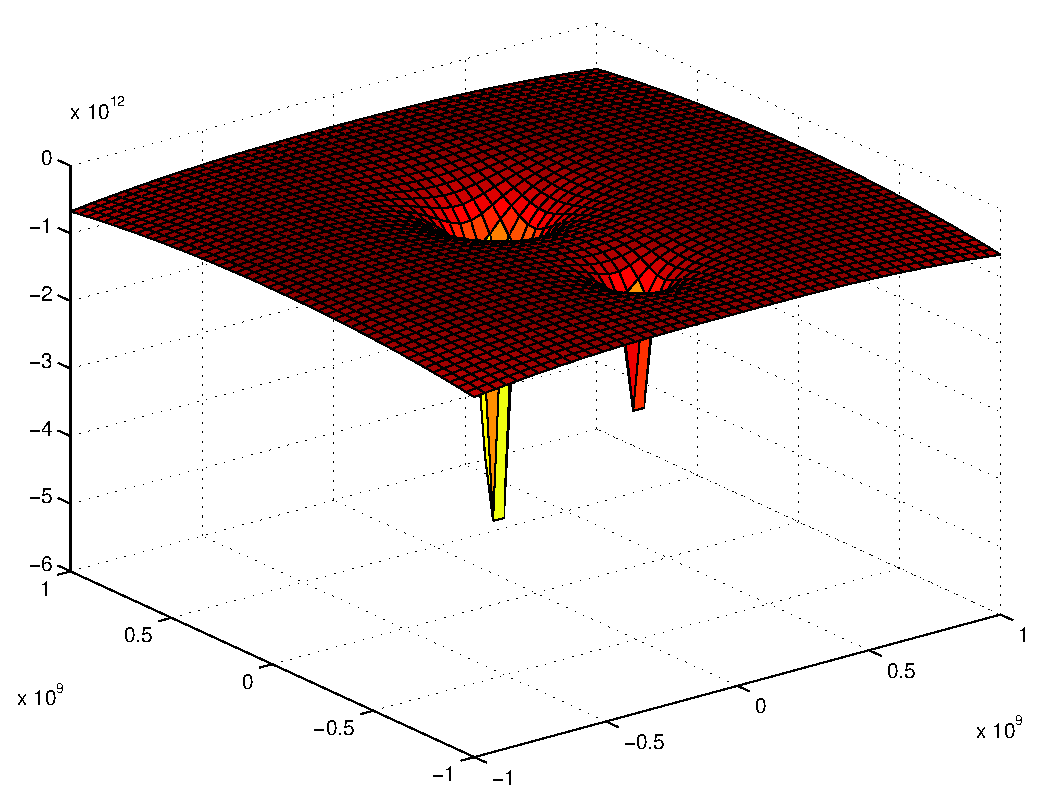
\includegraphics[scale=.35]{images/surf.eps}
    \end{center}
    \caption[Den vänstra figuren.]{Den vänstra figuren är den som är
      till vänster om den högra.}
\label{fig:leftfig}
  \end{minipage}\hfill
  \begin{minipage}[htb]{0.48\linewidth}
    \begin{center}
      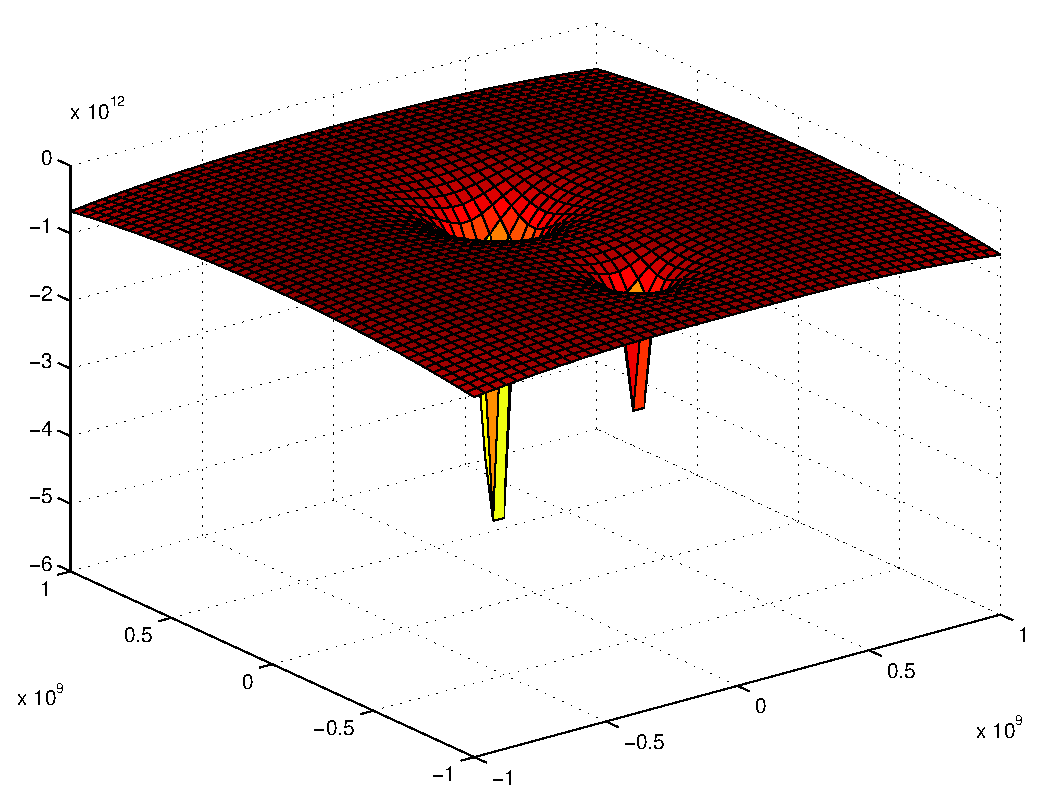
\includegraphics[scale=.35]{images/surf.eps}
    \end{center}
    \caption[Den högra figuren.]{Den högra figuren är den som är
      till höger om den vänstra.}
\label{fig:rightfig}
  \end{minipage}
\end{figure}

\begin{figure}[htb]
  \begin{center}
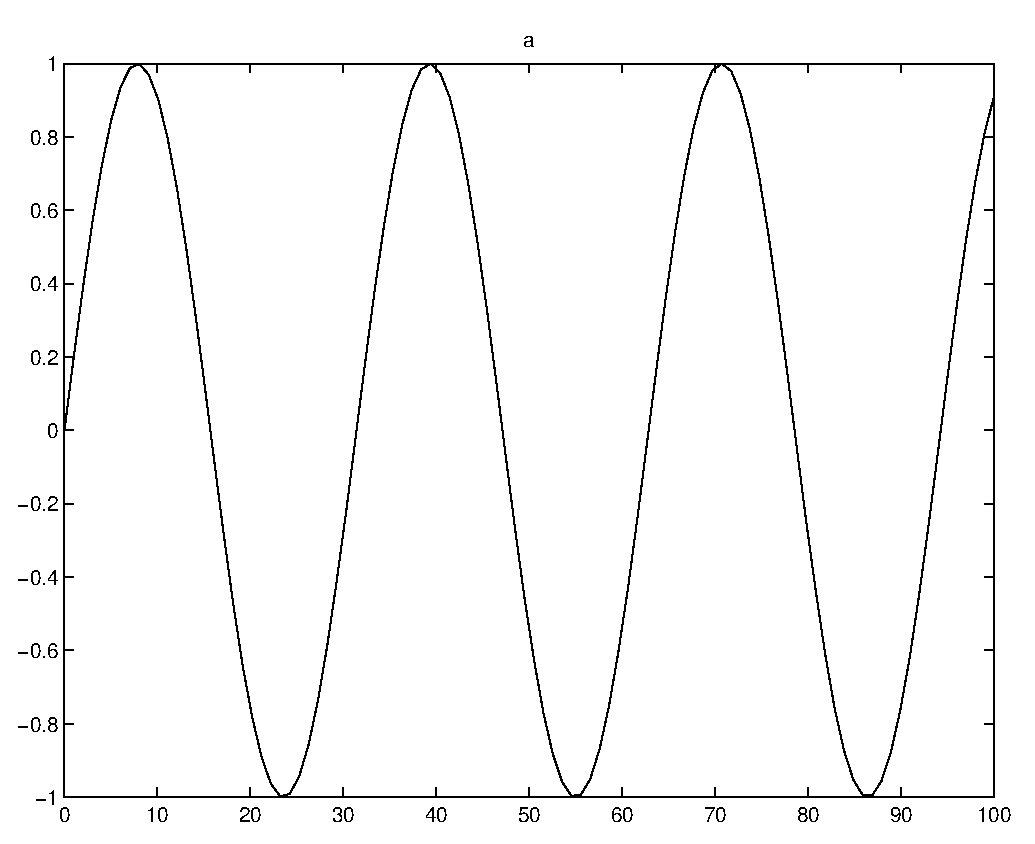
\includegraphics[width=0.8\linewidth]{images/sin.eps}
  \end{center}
  \caption[En ensam figur.]{En ensam figur mitt i sidan.}
\label{fig:center}
\end{figure}

\begin{figure}[!htb]
%\begin{subfigures}
  \begin{minipage}[htb]{0.48\linewidth}
    \begin{center}
      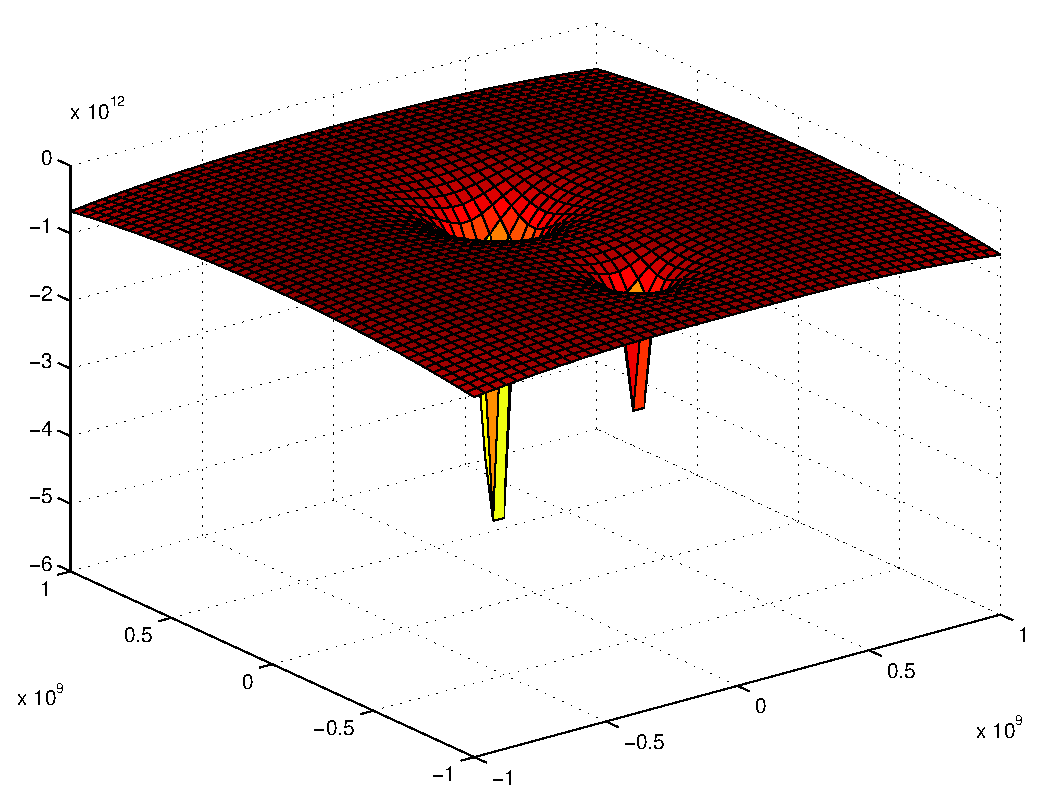
\includegraphics[scale=.35]{images/surf.eps}
    \end{center}
    \caption[Den vänstra figuren.]{Den vänstra figuren är den som är
      till vänster om den högra.}
\label{fig:leftfig2}
  \end{minipage}\hfill
  \begin{minipage}[htb]{0.48\linewidth}
    \begin{center}
      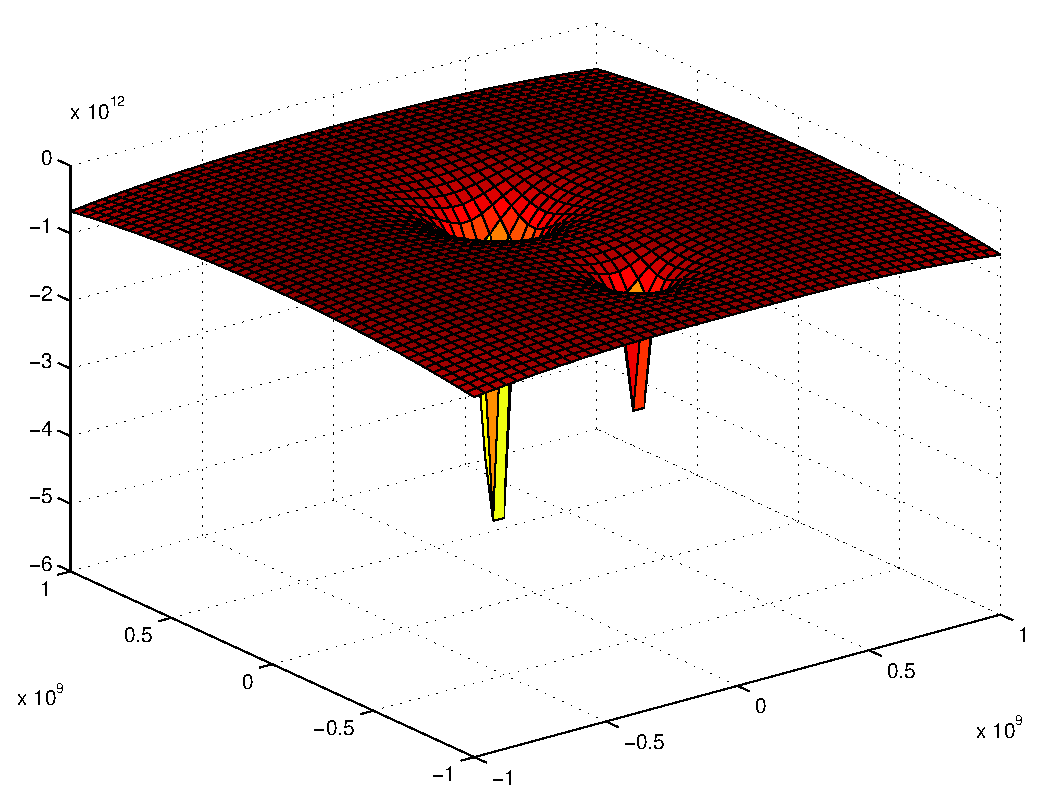
\includegraphics[scale=.35]{images/surf.eps}
    \end{center}
    \caption[Den högra figuren.]{Den högra figuren är den som är
      till höger om den vänstra.}
\label{fig:rightfig2}
  \end{minipage}
%\end{subfigures}
\end{figure}

\subsection{Ekvationer}
\label{subsec:eq}
Ekvationer kan nu ha sub-index.

\begin{subequations}
\begin{align}
a & = b \label{eq:a} \\
c &= d, \label{eq:b}
\end{align}
\end{subequations}

eller vara helt vanliga

\begin{equation}
  \lim_{n \to \infty}2\frac{E_{n+1}-E_{n}}{E_{n+1}+E_{n}}=0.
\label{eq:limn}
\end{equation}
\subsubsection{Spännande saker i ekvationer}
\label{subsubsec:spannend}
\begin{equation}
 A(n)\xrightarrow[n\to\infty]{}0
\end{equation}

\subsection{Tabeller}
\begin{table}
  \begin{center}
  \caption[Energier vid olika kvanttal]{Energier vid olika kvanttal ($1$ H $\approx$ $27.2$ eV)}
    \begin{tabular}{cc}\toprule
      $n$ & $E_n$ [Hartree]\\ \midrule
      $1$ & $1.23$ \\
      $2$ & $4.93$ \\
      $3$ & $11.10$\\
      $4$ & $19.74$\\
      $5$ & $30.84$\\
      $6$ & $44.41$\\
      $7$ & $60.45$\\
      $8$ & $78.96$\\
      $9$ & $99.93$\\
      $10$ &$123.37$\\ \bottomrule
    \end{tabular}

\label{tbl:energy}
  \end{center}
\end{table}

\subsection{Referenser och andra små ting}
\label{subsec:ref}

Man kan referera till ekvationer enligt Ekvation \eqref{eq:a}, till figurer och tabeller enligt Tabell \ref{tbl:energy} och till någon källa så här\cite{lshort}.

\itauthquote{Do you really believe the moon is not there if nobody looks?}{Albert Einstein (citerad av Pasqual Jordan)}

Citat som det ovan är en del av paketet \texttt{martin}.

\section{Kolumner}
\begin{multicols}{2}[\subsection{2 Kolumner}]
Lorem ipsum dolor sit amet, consectetuer adipiscing elit. Aliquam adipiscing gravida odio. Donec non ipsum non tellus egestas tincidunt. In ullamcorper. Phasellus massa eros, malesuada vel,  auctor mattis, lobortis nec, quam. Mauris vel lacus. Mauris volutpat ante nec nibh. Donec faucibus varius lorem. Maecenas rhoncus volutpat tortor. Sed nunc. Nam est risus, facilisis a, sollicitudin ut, pretium eu, lectus. Donec scelerisque mi at mi. Cras adipiscing. Pellentesque habitant morbi tristique senectus et netus et malesuada fames ac turpis egestas. Quisque risus. Etiam justo risus, tincidunt ac, faucibus ut, convallis id, pede. Praesent non ligula sit amet augue lobortis cursus.
\end{multicols}

%\section{Rotating}
%
%\begin{sideways} Lorem ipsum dolor sit amet. \end{sideways}
%\begin{turn}{45} Lorem ipsum dolor sit amet.\end{turn}
%\begin{rotate}{30} Praesent non ligula sit amet augue lobortis cursus.\end{rotate}
%\turnbox{-15}{Praesent non ligula sit amet augue lobortis cursus.}